\cleardoublepage\phantomsection
\phantomsection\mtcaddchapter[Anexo A: información suplementaria]
\FormatoAnexoA

%Agrego las marcas laterales
\AddLabelsAxUno

%Problemas con el tema del fancystyle
\let\originalstyle=\thispagestyle            % Store the command for later reuse.
\def\thispagestyle#1{\fancyfoot[C]{}}       % This clears footer in the center if fancyhdr is in use.
\def\thispagestyle#1{\originalstyle{empty}} % Use this to get blank header+footer, TeXnically it is only \thispagestyle{empty}.
\def\thispagestyle#1{}                       % This line completely ignores the content of the \thispagestyle command.

%Esto cambia el contador de las figuras para que coloque la letra del apendice
\renewcommand\thefigure{A.\arabic{figure}} 

\chapter*{Anexo A: información suplementaria}
  
  
    Se agregan en éste anexo los gráficos, imágenes y espectros que fueron apartados del cuerpo principal de la tesis. 

    \subsection*{Figuras correspondientes al capitulo \ref{chap:Mesoporosos}}

    %Simplificado

    	%Microscopia F127 Simplificado
      \begin{figure}[th]
		 	   	    \begin{subfigure}[t]{0.49\textwidth}
			       	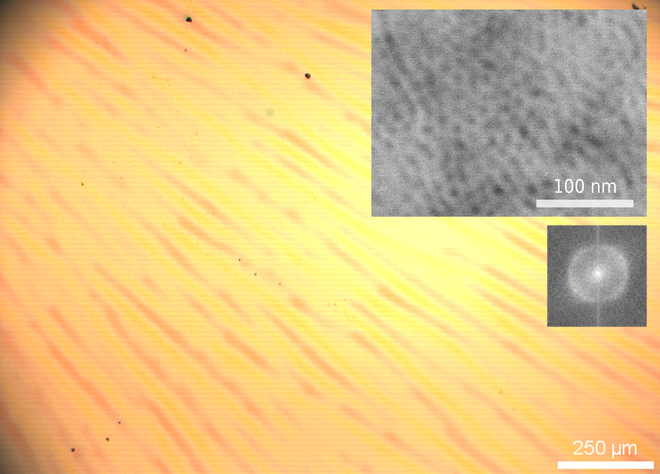
\includegraphics[width=\textwidth]{Imagenes/Au_EtF127-Combinada.jpg}
			   		\end{subfigure}
			   		\begin{subfigure}[t]{0.49\textwidth}
			   	    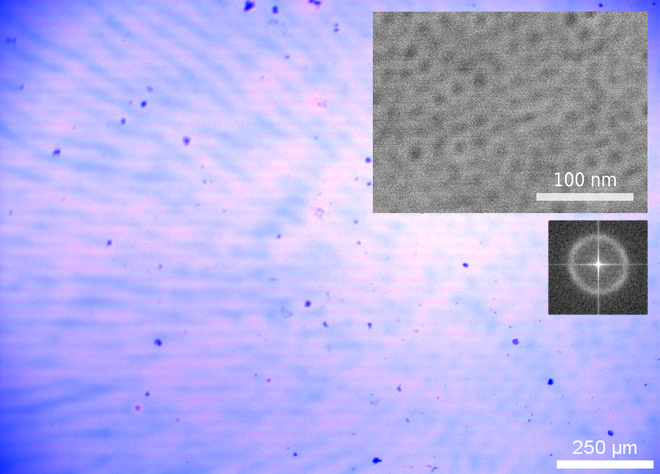
\includegraphics[width=\textwidth]{Imagenes/Si_EtF127-Combinada.jpg}
			   		\end{subfigure}
					 \caption[Microscopías \pdmF\space tratamiento simplificado.]{Microscopías ópticas para \pdmF\space sintetizadas por el tratamiento simplificado. Izquierda: sobre sustrato de Au. Derecha: sobre sustrato de Si. En los respectivos recuadros se observa el detalle por MEB del arreglo nanoporoso.}
					 \label{fig:Microscopia_F127_simplificado}	
				     \end{figure}		
	
		%Microscopia CTAB Simplificado
	  \begin{figure}[th]
 	   	    \begin{subfigure}[t]{0.49\textwidth}
	       	\includegraphics[width=\textwidth]{Imagenes/Au_EtCTAB-Combinada.jpg}
	   		\end{subfigure}
	   		\begin{subfigure}[t]{0.49\textwidth}
	   	    \includegraphics[width=\textwidth]{Imagenes/Si_EtCTAB-Combinada.jpg}
	   		\end{subfigure}
			 \caption[Microscopías \pdmC\space tratamiento simplificado.]{Microscopías ópticas para \pdmC\space sintetizadas por el tratamiento simplificado. Observese las grietas presentes cuando se sintetiza sobre Au (izquierda), mientras que sobre Si las \pdmC\space no presentan rupturas ni discontinuidades.}
			 \label{fig:Microscopia_CTAB_simplificado}	
		     \end{figure}	

		%Elipso F127 Simplificaco	     
	 \begin{figure}[th]
			  	\begin{subfigure}[t]{0.495\textwidth}
			  	\includegraphics[width=\textwidth]{Graficos/SI_F127_simplificado_EPA.pdf}
				\caption{Isorterma de adsorción/desorción de agua realizada por PEA para una \pdmF.}
				\label{fig:F127_simplificado_EPA}
				\end{subfigure}
				\begin{subfigure}[t]{0.495\textwidth}
			  	\includegraphics[width=\textwidth]{Graficos/SI_F127_simplificado_PSD.pdf}
				\caption{Distribución de tamaño de poro y cuello.\\ }
				\label{fig:F127_simplificado_PSD}
				\end{subfigure}
				\caption[Elipsoporosimetría \pdmF\space tratamiento simplificado.]{Resultados de elipsoporosimetría ambiental para una \pdmF\space sintetizada por el tratamientos simplificado.}
				\label{fig:F127_simplificado}
				\end{figure}
	
		%Elipso CTAB Simplificad
	 \begin{figure}[!ht]	
			\begin{subfigure}[t]{0.495\textwidth}
		  	\includegraphics[width=\textwidth]{Graficos/SI_CTAB_simplificado_EPA.pdf}
			\caption{Isorterma de adosroción/desorción de agua ralizada por PEA para una \pdmC.}
			\label{fig:CTAB_simplificado_EPA}
			\end{subfigure}
			\begin{subfigure}[t]{0.495\textwidth}
		  	\includegraphics[width=\textwidth]{Graficos/SI_CTAB_simplificado_PSD.pdf}
			\caption{Distribución de tamaño de poro y cuello.\\ }
			\label{fig:CTAB_simplificado_PSD}
			\end{subfigure}
			\caption[Elipsoporosimetría \pdmC\space tratamiento simplificado.]{Resultados de elipsoporosimetría ambiental para una \pdmC\space sintetizada por el tratamientos simplificado.}
			\end{figure}			

		%FTIR Simplificado		
	 \begin{figure}[ht]
				\begin{center}
				\includegraphics[width=0.75\textwidth]{Graficos/IR_F127_simplificado.pdf}
				\caption[FTIR \pdmF\space tratamiento simplificado.]{Espectro de absorción en el IR para una \pdmF\space sintetizada con el tratamiento simplificado antes y después de extraer el surfactante. Desaparece la banda de estiramiento C-H correspondiente al surfactante luego de la extarcción.}
				\label{fig:IR_F127_simplificado}
				\end{center}
				\end{figure}

		%FTIR Simplificado
	 \begin{figure}[!ht]
			\begin{center}
			\includegraphics[width=0.75\textwidth]{Graficos/IR_CTAB_simplificado.pdf}
			\caption[FTIR \pdmC\space tratamiento simplificado.]{Espectro de absorción en el IR para una \pdmC\space sintetizada con el tratamiento simplificado antes y después de extraer el surfactante. Todavía se puede apreciar un cantidad pequeña de surfactante luego de la extracción.}
			\label{fig:IR_CTAB_simplificado}
			\end{center}
			\end{figure}	

	%Prolongado
	
		%Microscopia F127 Prolongado
			 \begin{figure}[th]
		 	   	    \begin{subfigure}[t]{0.49\textwidth}
			       	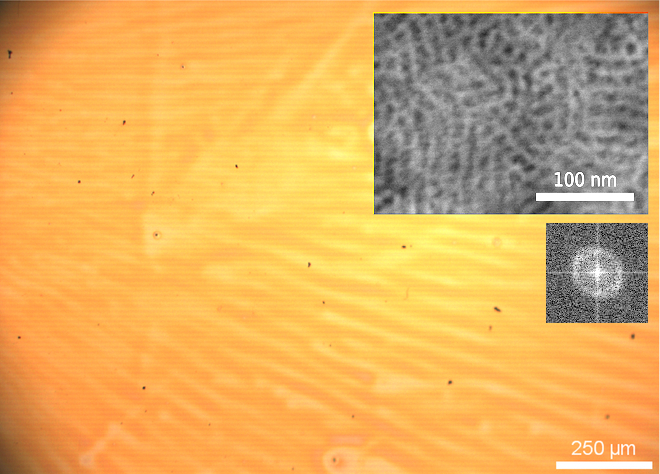
\includegraphics[width=\textwidth]{Imagenes/Au_130F127-Combinada.jpg}
			   		\end{subfigure}
			   		\begin{subfigure}[t]{0.49\textwidth}
			   	    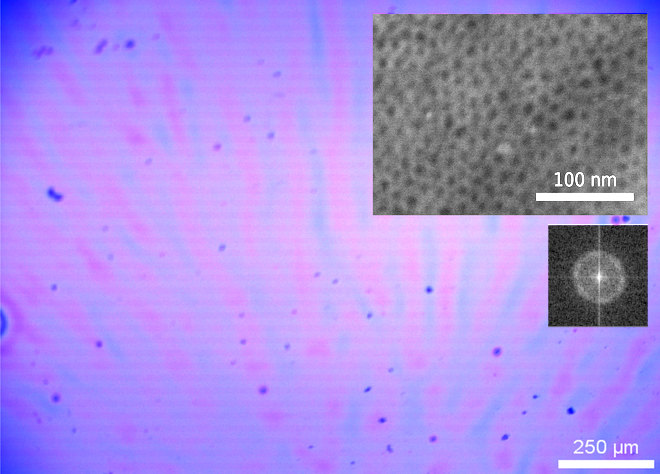
\includegraphics[width=\textwidth]{Imagenes/Si_130F127-Combinada.jpg}
			   		\end{subfigure}
					 \caption[Microscopía \pdmF\space tratamiento prolongado.]{Microscopías ópticas para \pdmF\space sintetizadas por el tratamiento prolongado. Izquierda: sobre sustrato de Au. Derecha: sobre sustrato de Si. En los respectivos recuadros se observa el detalle por MEB del arreglo nanoporoso.}
					 \label{fig:Microscopia_F127_prolongado}	
				     \end{figure}	

		%Microscopia CTAB Prolongado
		 \begin{figure}[!th]
	 	   	    \begin{subfigure}[t]{0.49\textwidth}
		       	\includegraphics[width=\textwidth]{Imagenes/Au_130CTAB-Combinada.jpg}
		   		\end{subfigure}
		   		\begin{subfigure}[t]{0.49\textwidth}
		   	    \includegraphics[width=\textwidth]{Imagenes/Si_130CTAB-Combinada.jpg}
		   		\end{subfigure}
				 \caption[Microscopía óptica \pdmC\space tratamiento prolongado.]{Microscopías ópticas para \pdmC\space sintetizadas por el tratamiento prolongado. Derecha: sobre sustrato de Au. Izquierda: sobre sustrato de Si.}
				 \label{fig:Microscopia_CTAB_prolongado}	
			     \end{figure}

		%Elipso F127 Prolongado
			 \begin{figure}[!ht]
			  	\begin{subfigure}[t]{0.495\textwidth}
			  	\includegraphics[width=\textwidth]{Graficos/SI_F127_prolongado_EPA.pdf}
				\caption{Isoterma de adsorción/desorción de agua realizada por PEA para \pdmF.}
				\label{fig:F127_prolongado_EPA}
				\end{subfigure}
				\begin{subfigure}[t]{0.495\textwidth}
			  	\includegraphics[width=\textwidth]{Graficos/SI_F127_prolongado_PSD.pdf}
				\caption{Distribución de tamaño de poro y cuello.\\ }
				\label{fig:F127_prolongado_PSD}
				\end{subfigure}
				\caption[Elipsoporosimetría \pdmF\space tratamiento prolongado.]{Resultados de PEA para sistema \pdmF\space sintetizada por el tratamientos prolongado, consistente en estabilización en humedad seguido de condensación por 7 días a \SI{130}{\celsius} y extracción.}
		 		\end{figure}

		%Elipso CTAB Prolongado
		 \begin{figure}[!ht]
		  	\begin{subfigure}[t]{0.495\textwidth}
		  	\includegraphics[width=\textwidth]{Graficos/SI_CTAB_prolongado_EPA.pdf}
			\caption{Isoterma de adosroción/desorción de agua ralizada por PEA para \pdmC\space.}
			\label{fig:CTAB_prolongado_EPA}
			\end{subfigure}
			\begin{subfigure}[t]{0.495\textwidth}
		  	\includegraphics[width=\textwidth]{Graficos/SI_CTAB_prolongado_PSD.pdf}
			\caption{Distribución de tamaño de poro y cuello.\\ }
			\label{fig:CTAB_prolongado_PSD}
			\end{subfigure}
			\caption[Elipsoporosimetría \pdmC\space tratamiento prolongado.]{Resultados de PEA para sistema \pdmC\space sintetizada por el tratamientos prolongado, consistente en estabilización en humedad seguido de condensación por 7 días a \SI{130}{\celsius} y extracción.}
			\end{figure}

		%FTIR F127 Prolongado
	
	  \begin{figure}[!ht]
			\begin{center}
			\includegraphics[width=0.75\textwidth]{Graficos/IR_F127_prolongado.pdf}
			\caption[FTIR \pdmF\space tratamiento prolongado.]{Espectro de absorción de IR correspondiente a una \pdmF\space sintetizada por el tratamiento prolongado antes y después de la extracción con 2-propanol.}
			\label{fig:IR_F127_prolongado}
			\end{center}
			\end{figure}
	
		%FTIR CTAB Prolongado	
		\begin{figure}[!ht]
			\begin{center}
			\includegraphics[width=0.75\textwidth]{Graficos/IR_CTAB_prolongado.pdf}
			\caption[FTIR \pdmC\space tratamiento prolongado.]{Espectro de absorción de IR correspondiente a una \pdmC\space sintetizada por el tratamiento prolongado antes y después de la extracción con 2-propanol.}
			\label{fig:IR_CTAB_prolongado}
			\end{center}
			\end{figure}		

  \let\thispagestyle=\originalstyle